\chapter{Appendix}
\section{Inventory of Resources}
\begin{table}[!ht]
    \caption{Inventory of Resources}
    \begin{tabular}{lll}
    \textbf{Type of resources} & \textbf{Kind of resources} & \textbf{Quantification}                                                    \\
    Personnel                  & business experts           & 1 person                                                                   \\
                               & data experts               & 1 person                                                                   \\
                               & technical support          & 1 person                                                                   \\
                               & data mining experts        & 1 person                                                                   \\
    Data                       & fixed extracts             & -                                                                \\
                               & live data                  & -                                                                          \\
                               & warehoused data            & -                                                                          \\
                               & operational data           & 1 dataset                                                                         \\
    Computing resources        & hardware platforms         & \begin{tabular}[c]{@{}l@{}}1 machine \\ access to SAP AI Core\end{tabular} \\
    Software                   & data mining tools          & anaconda, jupyter                                                          \\
                               & other relevant software    & Excel, Visual Studio Code, Git                                                                     
    \end{tabular}
    \label{tabelle:inventory}
    
    *) An asterisk indicates theoretical availability of more resources, if needed.
    \end{table}


\cleardoublepage


\section{Invoice Header Data}
\begin{multicols}{2}
	\label{invoice-header}
	\begin{itemize}
		\setlength\multicolsep{0pt}
		\item[] accountNumber.key
		\item[] accountNumber.value
		\item[] barCode.value
		\item[] buyerAddress.cityTownVillage.value
		\item[] buyerAddress.country.value
		\item[] buyerAddress.district.value
		\item[] buyerAddress.extraName.value
		\item[] buyerAddress.full.key
		\item[] buyerAddress.full.value
		\item[] buyerAddress.houseNumber.value
		\item[] buyerAddress.stateProvince.value
		\item[] buyerAddress.street.value
		\item[] buyerAddress.zip.value
		\item[] buyerName.key
		\item[] buyerName.value
		\item[] comments.key
		\item[] comments.value
		\item[] country.value
		\item[] currency.key
		\item[] currency.value
		\item[] deliveryDate.key
		\item[] deliveryDate.value
		\item[] deliveryNoteNo.key
		\item[] deliveryNoteNo.value
		\item[] discount.key
		\item[] discount.value
		\item[] dueDate.key
		\item[] dueDate.value
		\item[] employeeName.key
		\item[] employeeName.value
		\item[] exchRate.key
		\item[] exchRate.value
		\item[] exchRateSrcCurr.key
		\item[] exchRateSrcCurr.value
		\item[] exchRateTarCurr.key
		\item[] exchRateTarCurr.value
		\item[] filename
		\item[] index
		\item[] invoiceAmount.key
		\item[] invoiceAmount.value
		\item[] invoiceDate.key
		\item[] invoiceDate.value
		\item[] invoiceNo.key
		\item[] invoiceNo.value
		\item[] invoiceType.value
		\item[] language
		\item[] paymentTerms.key
		\item[] paymentTerms.value
		\item[] pii.address.key
		\item[] pii.address.value
		\item[] pii.email.key
		\item[] pii.email.value
		\item[] pii.name.key
		\item[] pii.name.value
		\item[] pii.other.key
		\item[] pii.other.value
		\item[] pii.phone.key
		\item[] pii.phone.value
		\item[] purchaseOrderNo.key
		\item[] purchaseOrderNo.value
		\item[] shipToAddress.cityTownVillage.value
		\item[] shipToAddress.country.value
		\item[] shipToAddress.district.value
		\item[] shipToAddress.extraName.value
		\item[] shipToAddress.full.key
		\item[] shipToAddress.full.value
		\item[] shipToAddress.houseNumber.value
		\item[] shipToAddress.stateProvince.value
		\item[] shipToAddress.street.value
		\item[] shipToAddress.zip.value
		\item[] shippingAmount.key
		\item[] shippingAmount.value
		\item[] subtotalAmount.key
		\item[] subtotalAmount.value
		\item[] tableHeader.batchNumber.value
		\item[] tableHeader.description.value
		\item[] tableHeader.discount.value
		\item[] tableHeader.materialNumber.value
		\item[] tableHeader.purchaseOrderNumber.value
		\item[] tableHeader.quantity.value
		\item[] tableHeader.serialNumber.value
		\item[] tableHeader.tableHeaderBox
		\item[] tableHeader.tax10Amount.value
		\item[] tableHeader.tax10Rate.value
		\item[] tableHeader.tax1Amount.value
		\item[] tableHeader.tax1Rate.value
		\item[] tableHeader.tax2Amount.value
		\item[] tableHeader.tax2Rate.value
		\item[] tableHeader.tax3Amount.value
		\item[] tableHeader.tax3Rate.value
		\item[] tableHeader.tax4Amount.value
		\item[] tableHeader.tax4Rate.value
		\item[] tableHeader.tax5Amount.value
		\item[] tableHeader.tax5Rate.value
		\item[] tableHeader.tax6Amount.value
		\item[] tableHeader.tax6Rate.value
		\item[] tableHeader.tax7Rate.value
		\item[] tableHeader.totalAmount.value
		\item[] tableHeader.unitOfMeasure.value
		\item[] tableHeader.unitPrice.value
		\item[] tax10Amount.key
		\item[] tax10Amount.value
		\item[] tax10Description.key
		\item[] tax10Description.value
		\item[] tax10Rate.key
		\item[] tax10Rate.value
		\item[] tax1Amount.key
		\item[] tax1Amount.value
		\item[] tax1Description.key
		\item[] tax1Description.value
		\item[] tax1Rate.key
		\item[] tax1Rate.value
		\item[] tax2Amount.key
		\item[] tax2Amount.value
		\item[] tax2Description.key
		\item[] tax2Description.value
		\item[] tax2Rate.key
		\item[] tax2Rate.value
		\item[] tax3Amount.key
		\item[] tax3Amount.value
		\item[] tax3Description.key
		\item[] tax3Description.value
		\item[] tax3Rate.key
		\item[] tax3Rate.value
		\item[] tax4Amount.key
		\item[] tax4Amount.value
		\item[] tax4Description.key
		\item[] tax4Description.value
		\item[] tax4Rate.key
		\item[] tax4Rate.value
		\item[] tax5Amount.key
		\item[] tax5Amount.value
		\item[] tax5Description.value
		\item[] tax5Rate.key
		\item[] tax5Rate.value
		\item[] tax6Amount.key
		\item[] tax6Amount.value
		\item[] tax6Description.key
		\item[] tax6Description.value
		\item[] tax6Rate.key
		\item[] tax6Rate.value
		\item[] tax7Amount.key
		\item[] tax7Amount.value
		\item[] tax7Description.value
		\item[] tax7Rate.key
		\item[] tax7Rate.value
		\item[] tax8Amount.key
		\item[] tax8Amount.value
		\item[] tax8Description.value
		\item[] tax8Rate.key
		\item[] tax8Rate.value
		\item[] tax9Amount.key
		\item[] tax9Amount.value
		\item[] tax9Description.value
		\item[] tax9Rate.key
		\item[] tax9Rate.value
		\item[] totalAmount.key
		\item[] totalAmount.value
		\item[] vendorAddress.cityTownVillage.value
		\item[] vendorAddress.country.value
		\item[] vendorAddress.district.value
		\item[] vendorAddress.extraName.value
		\item[] vendorAddress.full.key
		\item[] vendorAddress.full.value
		\item[] vendorAddress.houseNumber.value
		\item[] vendorAddress.stateProvince.value
		\item[] vendorAddress.street.value
		\item[] vendorAddress.zip.value
		\item[] vendorBankAccountNo.key
		\item[] vendorBankAccountNo.value
		\item[] vendorName.key
		\item[] vendorName.value
		\item[] vendorTaxID.key
		\item[] vendorTaxID.value
\end{itemize}
\end{multicols}
\cleardoublepage



\section{Invoice Line Item Data}
\begin{multicols}{2}
	\label{invoice-lines}
	\begin{itemize}
		\setlength\multicolsep{0pt}
		\item[] lineItem.batchNumber.value
		\item[] lineItem.description.value
		\item[] lineItem.discount.value
		\item[] lineItem.lineItemBox
		\item[] lineItem.materialNumber.value
		\item[] lineItem.purchaseOrderNumber.value
		\item[] lineItem.quantity.value
		\item[] lineItem.serialNumber.value
		\item[] lineItem.tax10Amount.value
		\item[] lineItem.tax10Rate.value
		\item[] lineItem.tax1Amount.value
		\item[] lineItem.tax1Rate.value
		\item[] lineItem.tax2Amount.value
		\item[] lineItem.tax2Rate.value
		\item[] lineItem.tax3Amount.value
		\item[] lineItem.tax3Rate.value
		\item[] lineItem.tax4Amount.value
		\item[] lineItem.tax4Rate.value
		\item[] lineItem.tax5Amount.value
		\item[] lineItem.tax5Rate.value
		\item[] lineItem.tax6Amount.value
		\item[] lineItem.tax6Rate.value
		\item[] lineItem.tax7Amount.value
		\item[] lineItem.tax7Rate.value
		\item[] lineItem.tax8Amount.value
		\item[] lineItem.tax8Rate.value
		\item[] lineItem.tax9Amount.value
		\item[] lineItem.tax9Rate.value
		\item[] lineItem.totalAmount.value
		\item[] lineItem.unitOfMeasure.value
		\item[] lineItem.unitPrice.value
	\end{itemize}
\end{multicols}
\newpage
\section{Benchmarking DataFrames and Dictionaries}

\label{benchmarkDF}
\begin{figure}[h!]
	%\left
	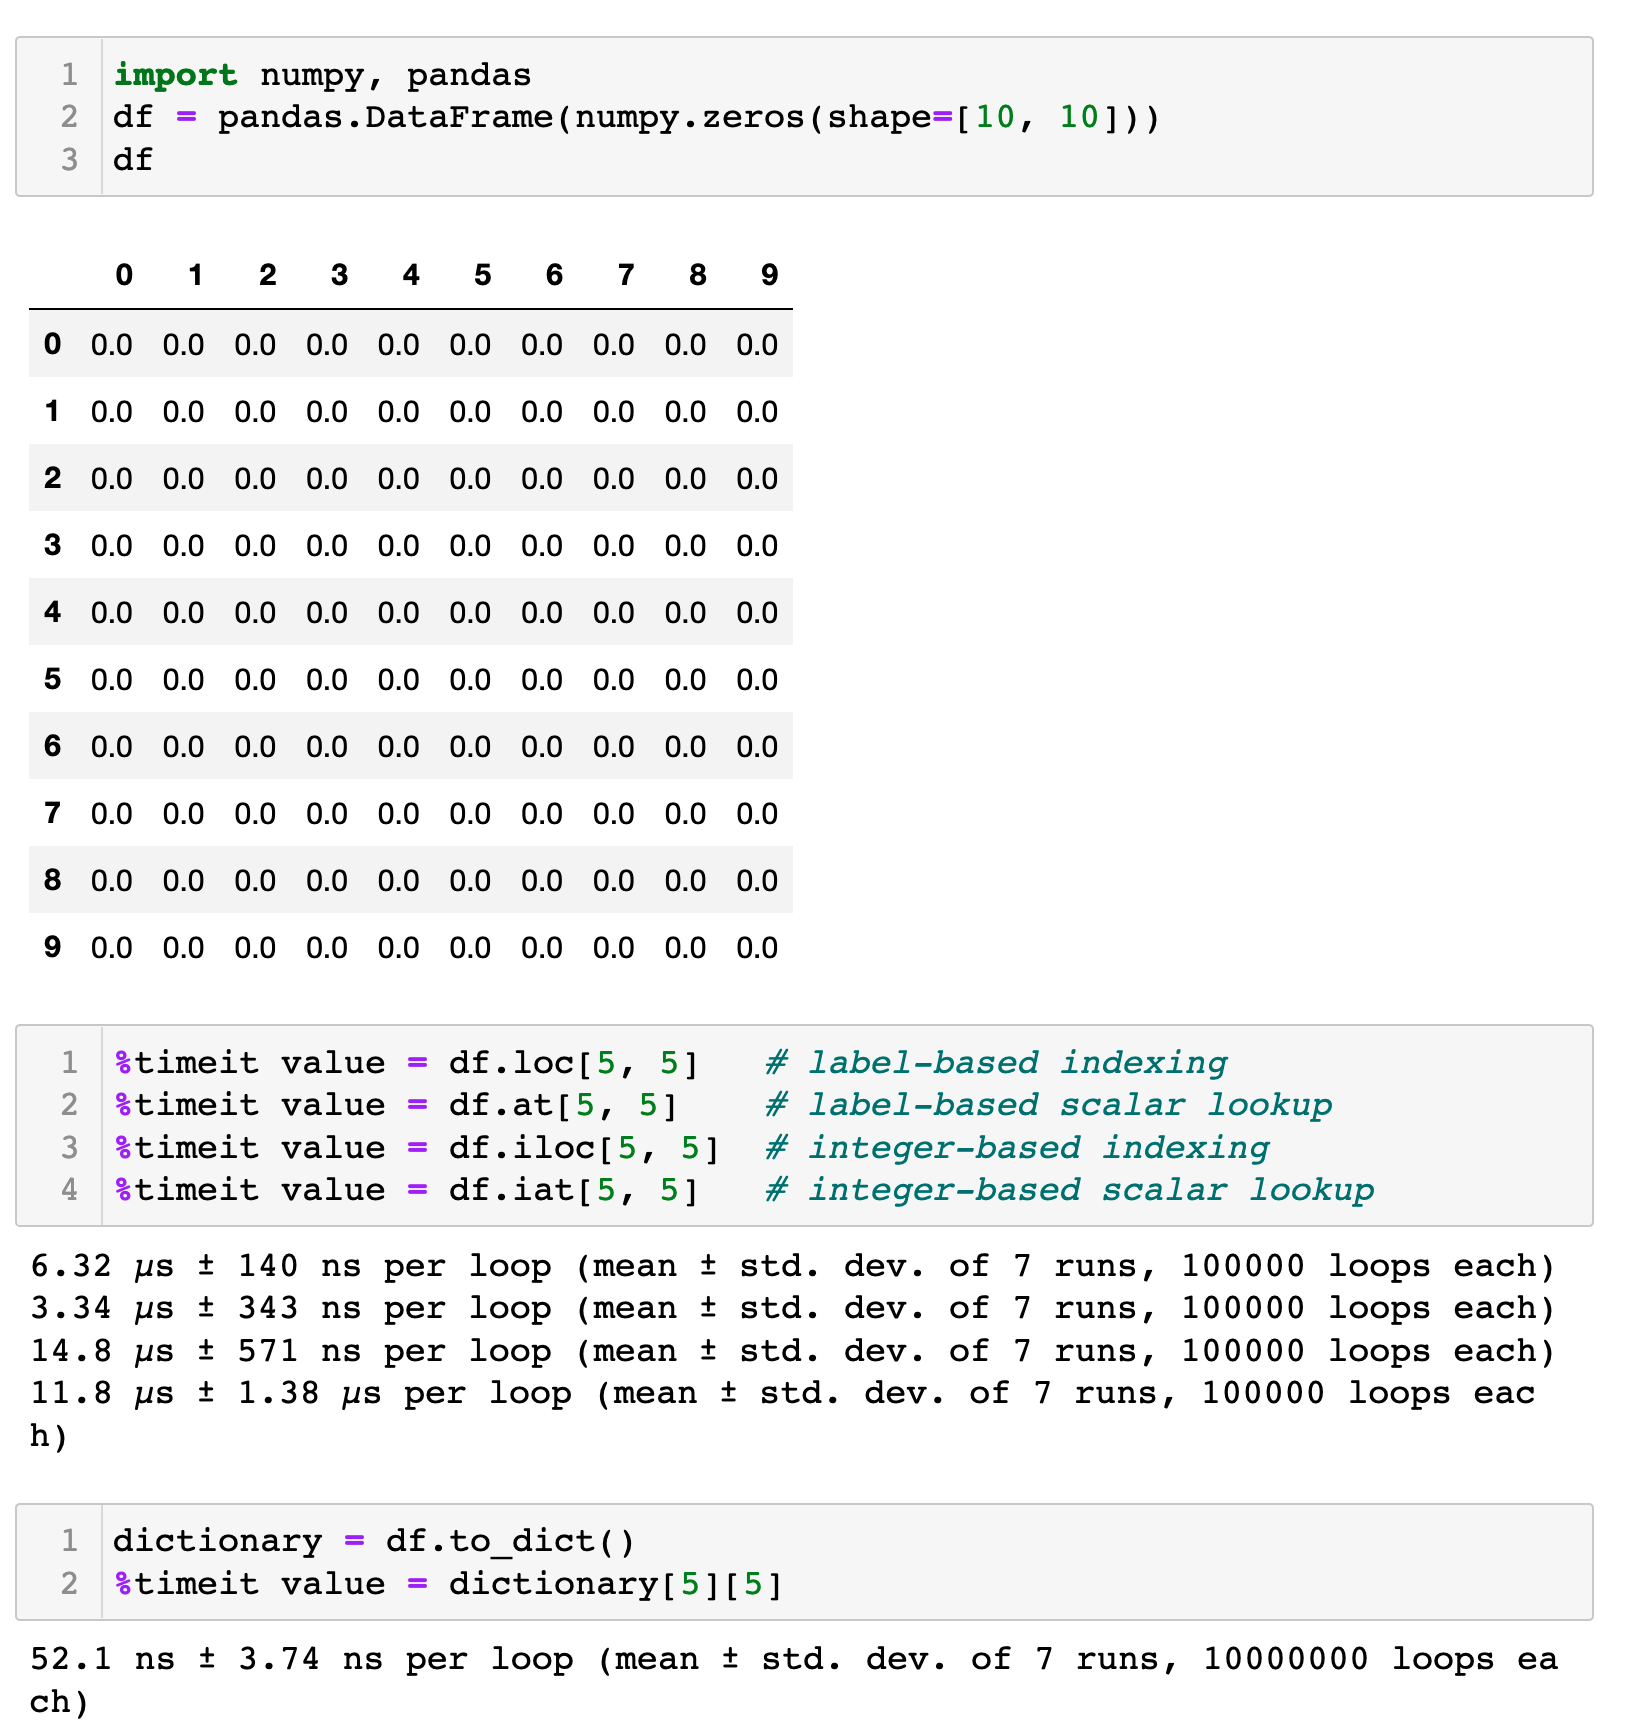
\includegraphics[height=15cm]{Bilder/appendix/dfvsdict.png}
	\label{fig:dbscan-plot}
\end{figure}
\begin{lstlisting}[caption={Benchmark of Indexing with Python Data Structures}]
	   
\end{lstlisting}
The \lstinline|.loc| indexing is  130.24 times slower than dictionary access.\\
The \lstinline|.at|  indexing is  62.06 times slower than dictionary access.\\
The \lstinline|.iloc|  indexing is  310.28 times slower than dictionary access.\\
The \lstinline|.iat|  indexing is  213.44 times slower than dictionary access.

\section{File Processing Script}
\lstinputlisting[
label=code:InvoiceReader,    % Label; genutzt für Referenzen auf dieses Code-Beispiel
caption=Python Script for extracting JSON Data into a DataFrame,
captionpos=b,               % Position, an der die Caption angezeigt wird t(op) oder b(ottom)
style=EigenerPythonStyle,   % Eigener Style der vor dem Dokument festgelegt wurde
firstline=0,                % Zeilennummer im Dokument welche als erste angezeigt wird
lastline=23                 % Letzte Zeile welche ins LaTeX Dokument übernommen wird
]{Quellcode/reader}


\section{\ac{TF-IDF}}
\label{appendix:tfidf}
\begin{figure}[]
	\centering
	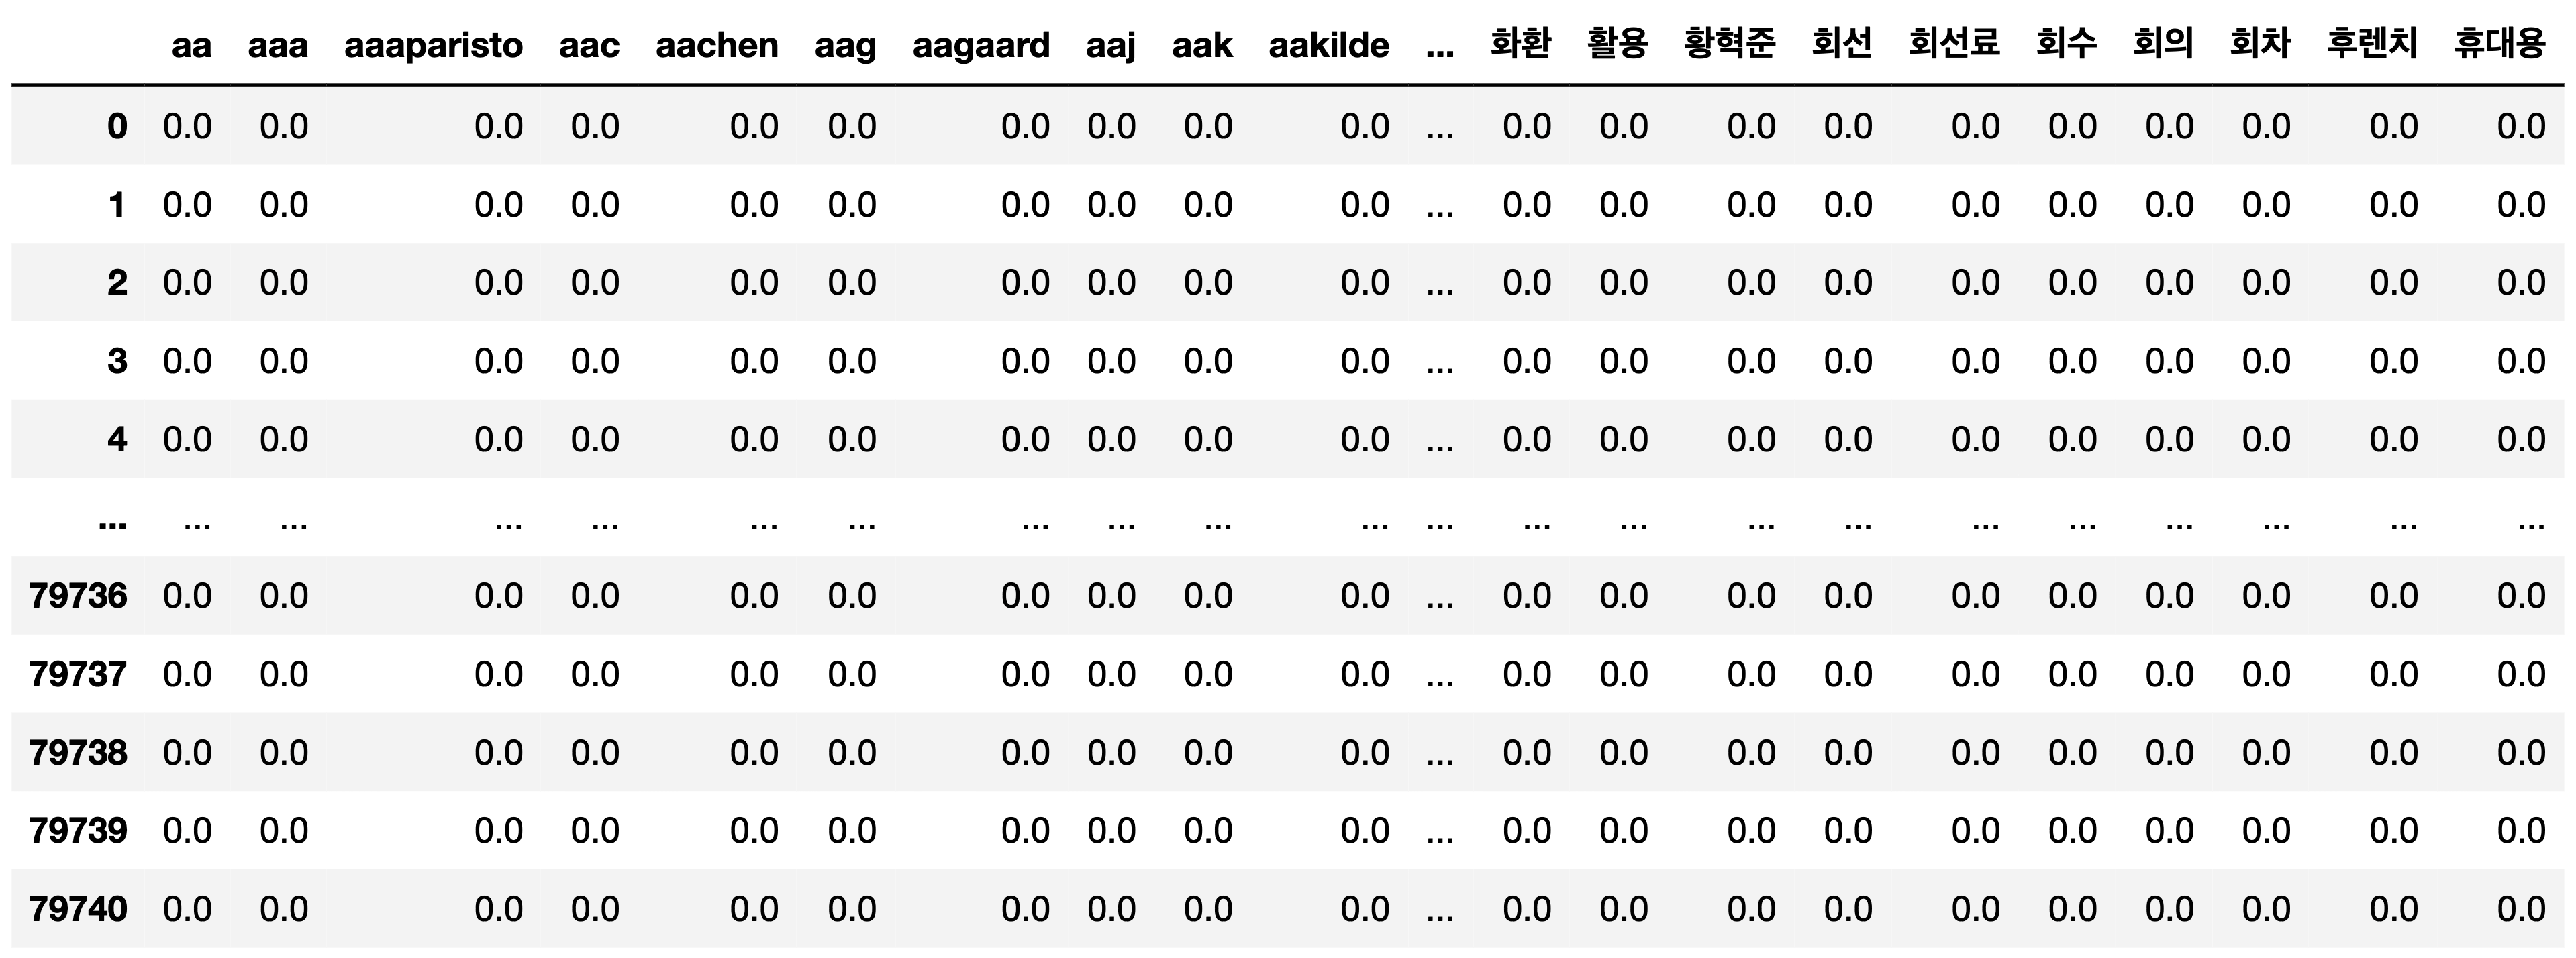
\includegraphics[height=6cm]{Bilder/preprocessing/tfidf.png}
	\label{fig:tfidf}
	\caption{Features extracted with TF-IDF}
\end{figure}
\begin{figure}[]
	\centering
	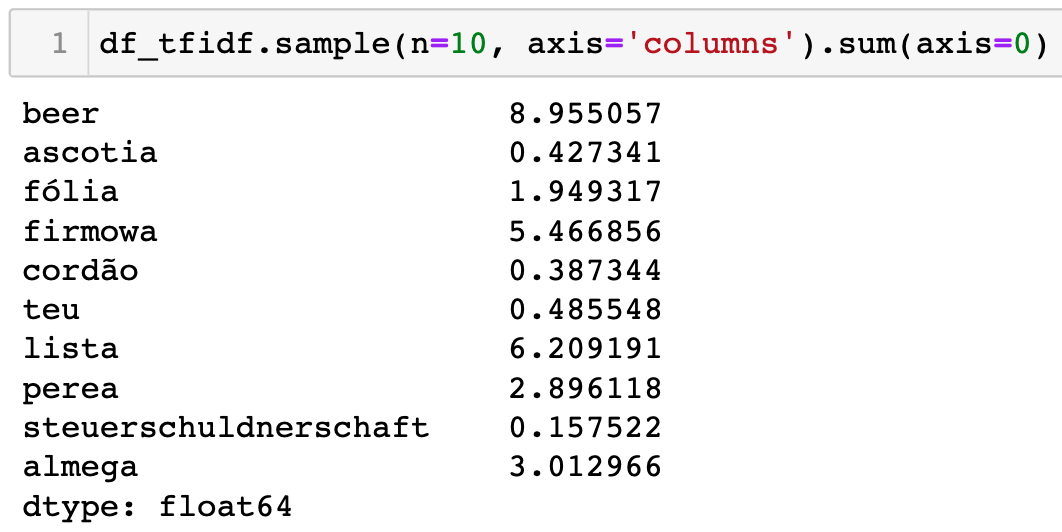
\includegraphics[height=6cm]{Bilder/preprocessing/tfidf_sparse.png}
	\label{fig:tfidf_sparse}
	\caption{Ten words from the Vocabulary and their summed Weight}
\end{figure}

\newpage

\section{Architectures for Learning Word Embeddings}
 \subparagraph{\aclu{CBOW}} 
With the \ac{CBOW} architecture the word2vec model is trained to predict a word using the context as input. A sliding window of a predefined size is moved along the text. 

\begin{figure}[ht]
	\centering
	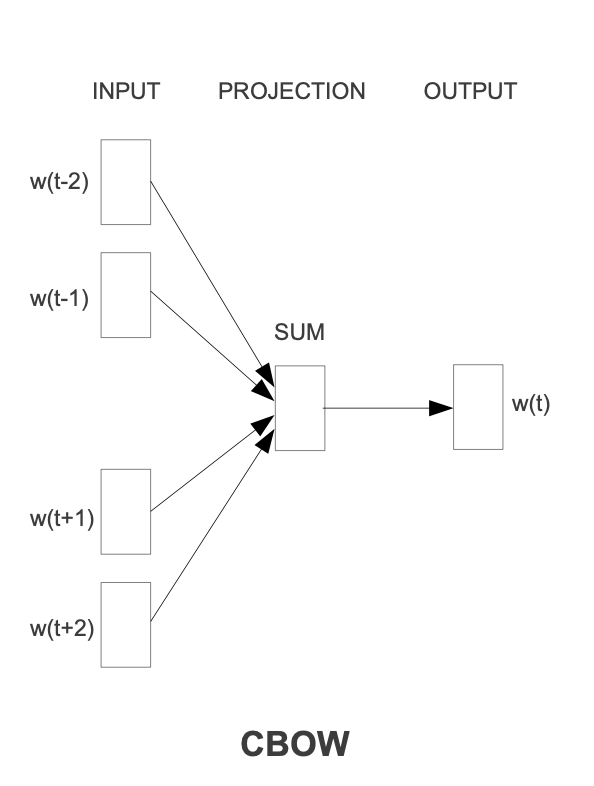
\includegraphics[height=6cm]{Bilder/word2vec/architecture_cbow.png}
	\caption{\aclu{CBOW} architecture\\\ with sliding window of size $C=5$ }
	\label{fig:cbow-architecture}
\end{figure}

\subparagraph{Skipgram} 
With the skipgram architecture the word2vec model is trained to predict the context of the input word.

\begin{figure}[ht]
	\centering
	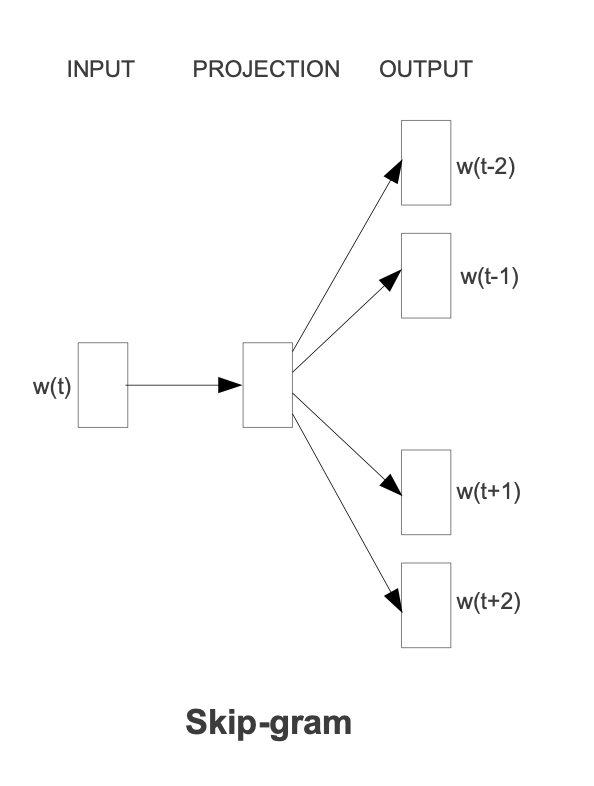
\includegraphics[height=6cm]{Bilder/word2vec/architecture_skipgram.png}
	\caption{Skipgram architecture\\\ with sliding window of size $C=5$ }
	\label{fig:skipgram-architecture}
\end{figure}

\begin{figure}[ht]
	\centering
	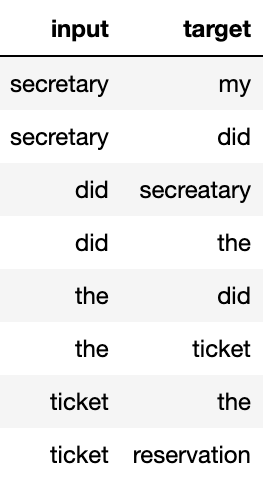
\includegraphics[height=8cm]{Bilder/word2vec/skipgram.png}
	\caption{Observations for training with skipgram architecture}
	
\end{figure}


\subparagraph{Negative Sampling}


Word2Vec uses either SKIPGram or CBOW.

Word2vec can utilize two models for selecting observations: either skipgram or \ac{CBOW}. 

\newpage
\section{Transformer Architecture}

\begin{figure}[h!]
	\label{fig:transformer}
	\centering
	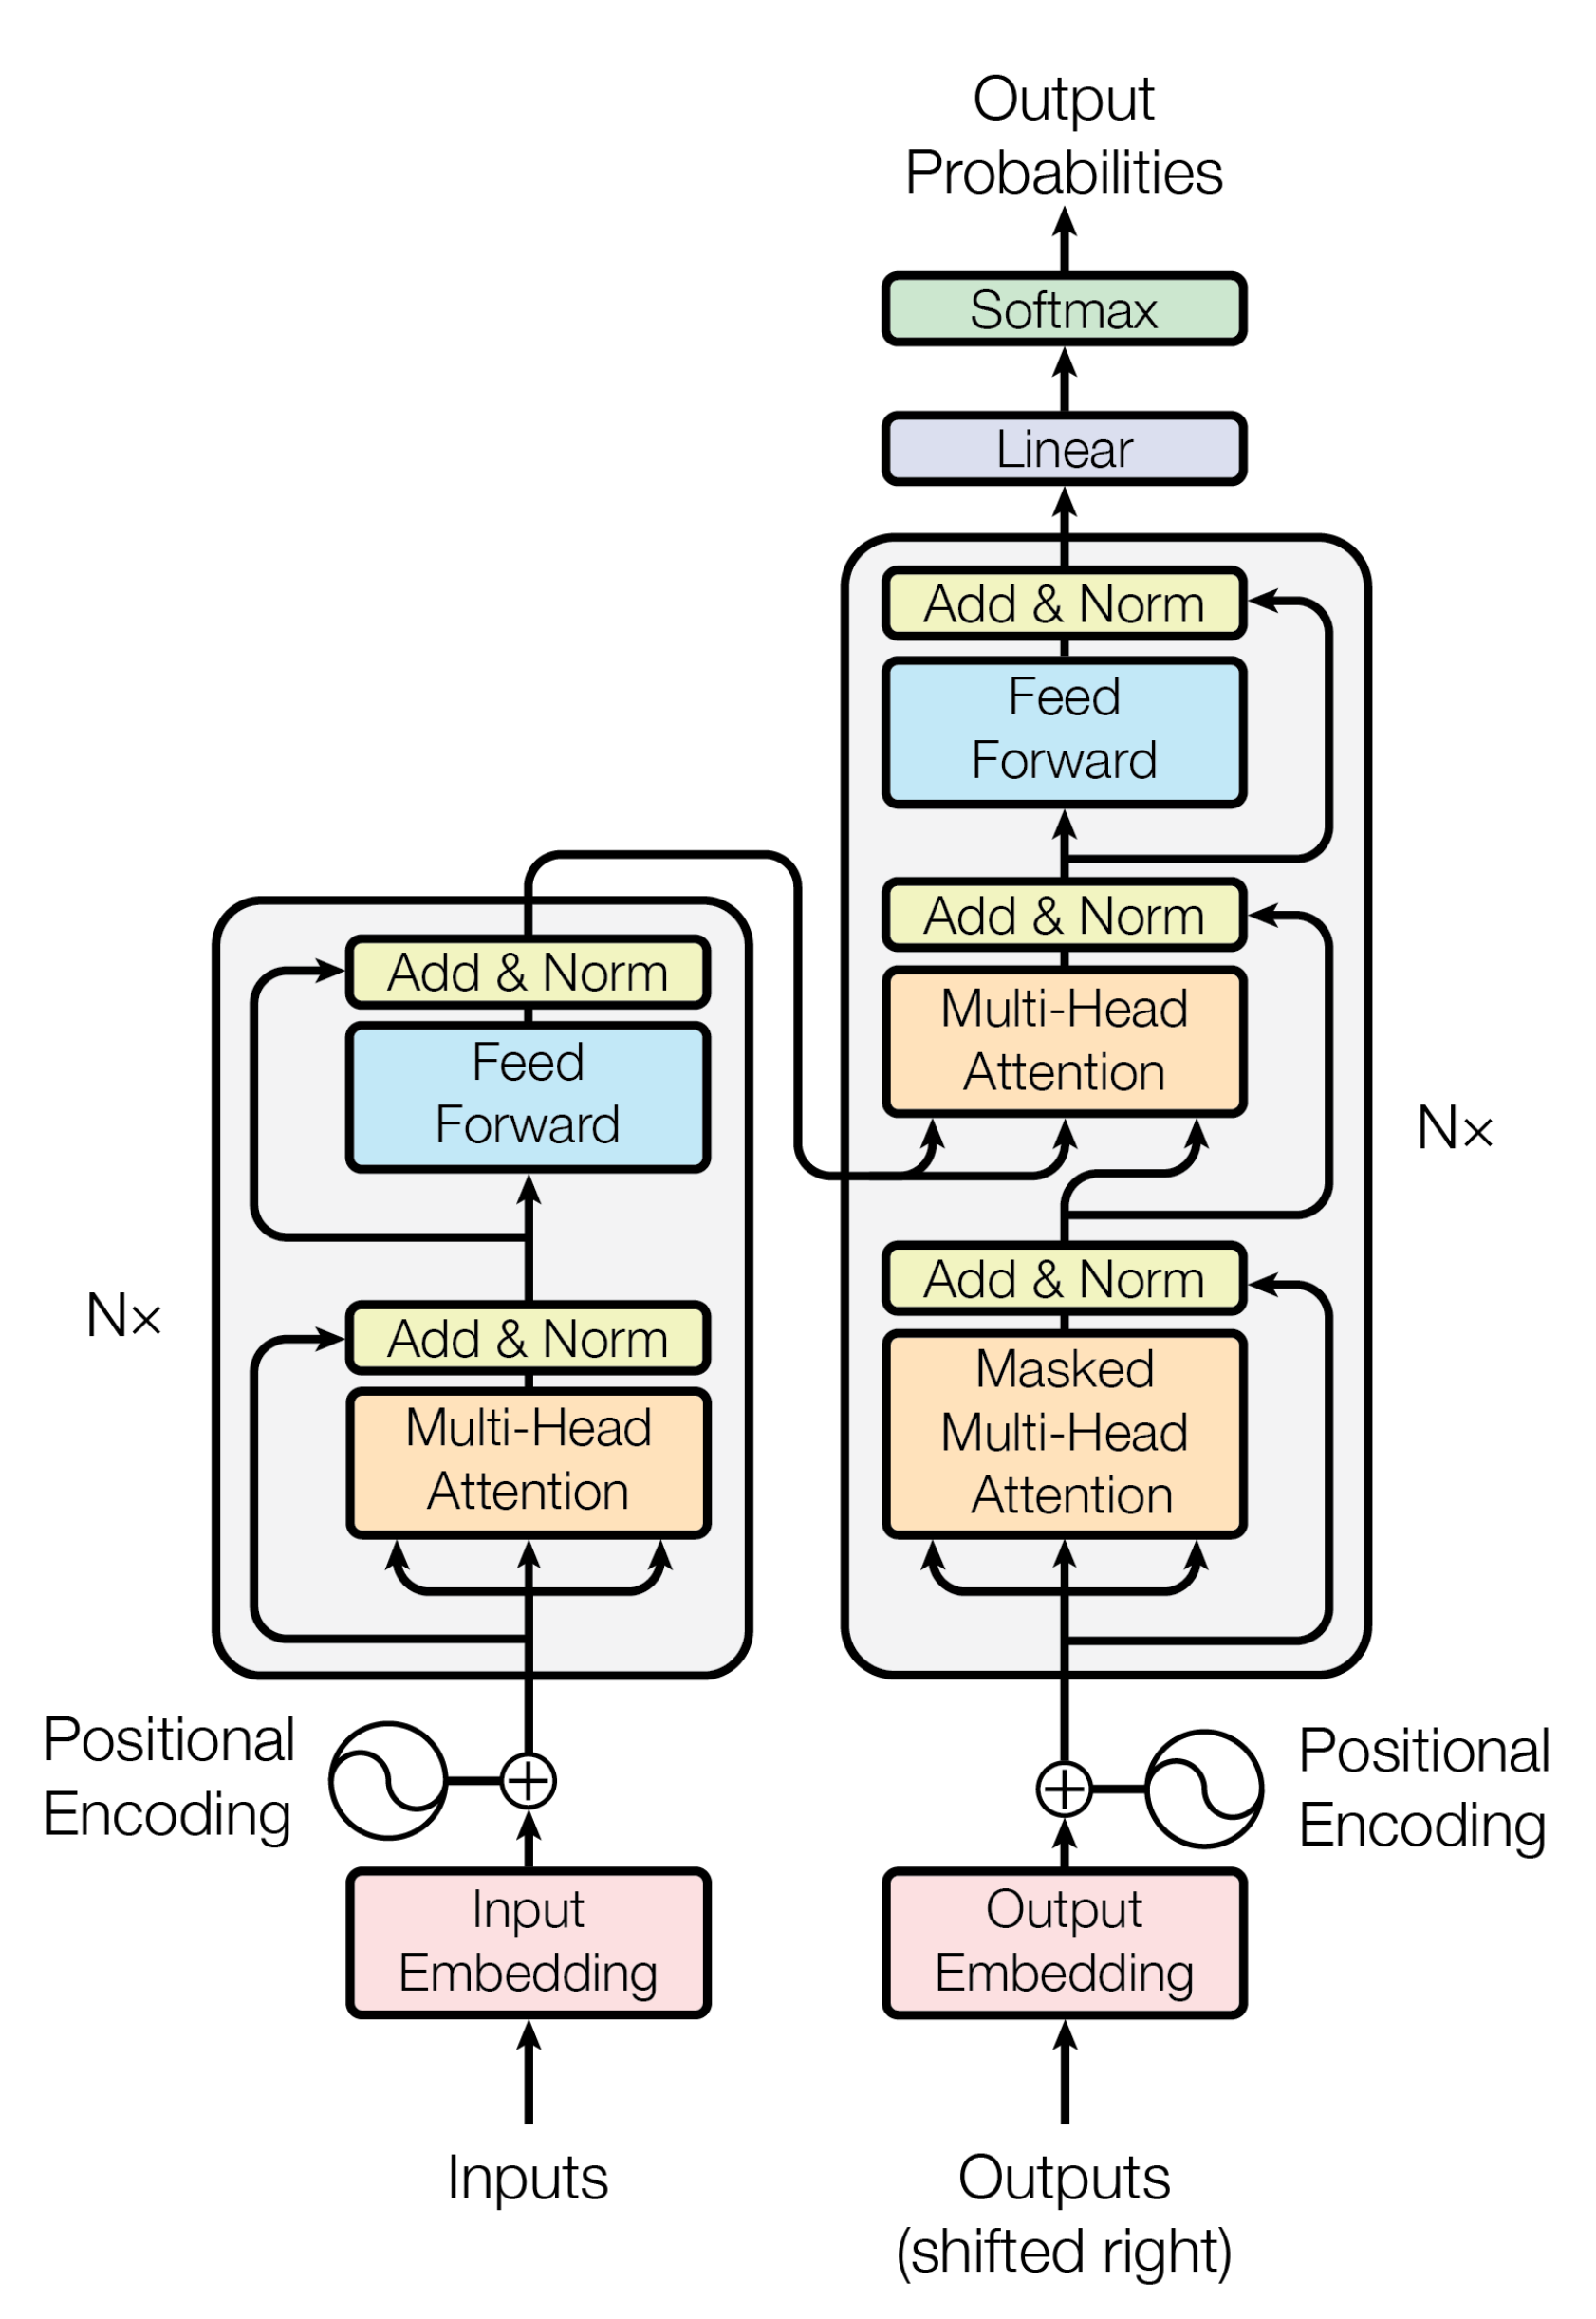
\includegraphics[height=18cm]{Bilder/preprocessing/BERT/transformer_architecture.png}
	\caption{Observations for training with skipgram architecture}
\end{figure}




\newpage
\section{Outliers}

\begin{figure}[h!]
	\centering
	\includegraphics[height=18cm]{Bilder/models/outliers.pdf}
	\caption{Projection of the Data with Outliers marked Red }
	\label{fig:dbscan-outliers}
\end{figure}